\documentclass[tikz]{standalone}
\usepackage{pgfplots}
\begin{document}
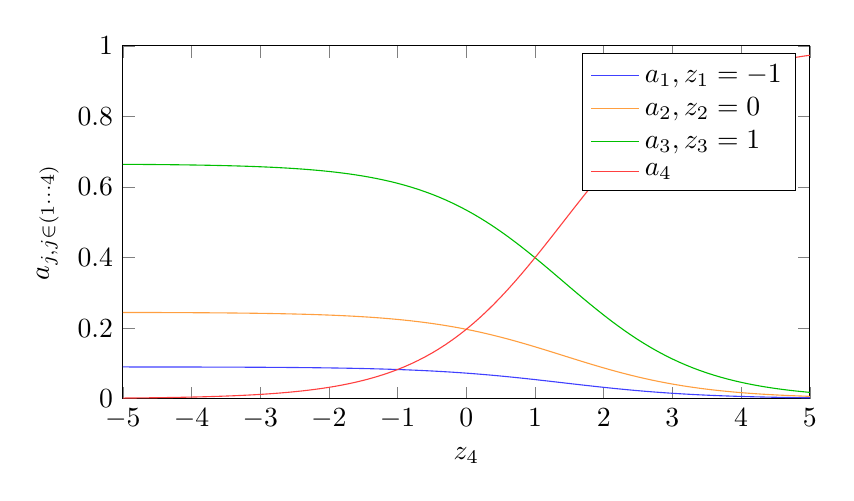
\begin{tikzpicture}
\begin{axis}[xmin=-5,xmax=5,ymin=0,ymax=1,xlabel={$z_4$},ylabel={$a_{j, j\in (1\cdots4)}$},width=0.85\linewidth,height=0.5\linewidth,legend cell align={left}]
	\addplot[domain=-5:5,samples=101,blue!75] {exp(-1)/(exp(x)+exp(1)+exp(0)+exp(-1))};
	\addplot[domain=-5:5,samples=101,orange!75] {exp(0)/(exp(x)+exp(1)+exp(0)+exp(-1))};
	\addplot[domain=-5:5,samples=101,green!75!black] {exp(1)/(exp(x)+exp(1)+exp(0)+exp(-1))};
	\addplot[domain=-5:5,samples=101,red!75] {exp(x)/(exp(x)+exp(1)+exp(0)+exp(-1))};
	\addlegendentry{$a_1,z_1=-1$};
	\addlegendentry{$a_2,z_2=0$};
	\addlegendentry{$a_3,z_3=1$};
	\addlegendentry{$a_4$};	
\end{axis}
\end{tikzpicture}
\end{document}
